% -- UMN Ph.D Thesis Template for modern Latex
% -- Designed to use modern packages and basic modifications to yield a flexible result
% -- Author: Ross S. Chaudhry, November 2018

% -- The most popular previous version uses a *lot* of hacks that should be done with modern packages.
% -- (https://github.com/agude/UMN-PhD-Thesis-Template)
% -- I found this made it difficult to customize,
% -- such as the page number locations, table style, geometry, and so on.

% -- Good links for development of this document:
%     ~ 'Writing a thesis with latex' https://tug.org/pracjourn/2008-1/mori/mori.pdf
%     ~ UMN latex template on github: https://github.com/agude/UMN-PhD-Thesis-Template
%     ~ Thesis format guidelines from the grad school: https://assets.asr.umn.edu/files/gssp/Thesis_formatting_guidelines.pdf

% -- main.tex includes all global formatting modifications
% -- Other sections are:

% -- Book class because it offers front, main, and backmatter commands
% -- Good discussion here: https://tex.stackexchange.com/questions/36988/regarding-the-book-report-and-article-document-classes-what-are-the-mai
% -- Uses the following settings:
%     ~ 11 pt font. Personally I think 10 is too small, which is the minimum of graduate school.
%     ~ oneside makes the geometry layout not dependent on parity (even-odd).
%       Grad school requires same layout for each page, although apparently it can be printed two-sided.
%       In this case, the printing firm modifies the layout (shift 0.5 in left).
%     ~ openany means chapters can begin on either right or left pages.
% -- Unfortunately, the requirements are incompatable with two-sided documents.
\documentclass[11 pt, oneside, openany, letterpaper]{book}

% ===== Declare all packages, and set settings for those packages
% -- Page geometry
% -- includefoot/includehead include the header and footer in main block, ie NOT margins
% -- If there is *nothing* inside the header, do not use includefoot
% -- But, if there are page numbers inside the header, use includefoot
% -- Same for head
% -- Choose to use page numbers in footer always, so *nothing* can go in header
\usepackage[letterpaper,
   top=1in,bottom=1in,
   inner=1.5in,outer=1in,
   includefoot]
   {geometry}

% -- Page numbering location, set to middle bottom the whole way
% -- Could use fancyhdr if more stuff was desired
\pagestyle{plain}

% -- Spacing of document, double or onehalf is allowed
\usepackage[onehalfspacing]{setspace}

% -- Configure the appendix, currently set to the following:
%     ~ titletoc     In the TOC, lists appendix as Appendix A
%       (title and header are set by default)
\usepackage[titletoc]{appendix}

% -- Essentials
\usepackage{hyperref}               % -- Makes headings and links clickable. Mandatory because \phantomsection command
\usepackage[utf8]{inputenc}
\usepackage{graphicx}
\usepackage{amsmath}

% -- Tables
\usepackage{booktabs}               % -- Pretty tables, provides \toprule, \midrule, bottomrule
\usepackage{multirow}
\usepackage{threeparttable}         % -- Footnotes and set-width captions for tables. Enables \tnote and threeparttable
% -- Symbol order (for *each* table)
% -- Symbol order should follow here: https://tex.stackexchange.com/questions/54899/looking-for-a-style-guideline-to-put-many-references-in-a-table
\newcommand{\mytna}{*}
\newcommand{\mytnb}{\textdagger}
\newcommand{\mytnc}{\textdaggerdbl}
\newcommand{\mytnd}{\S}
\newcommand{\mytne}{$\|$}
\newcommand{\mytnf}{$\!$\#}

% -- Longtable for glossary section
\usepackage{longtable}

% -- Citations and references
\usepackage[sort&compress,numbers]{natbib}
\usepackage[noabbrev, capitalize]{cleveref}  % -- \cref{myfig} looks like Figure~\ref{myfig}
\newcommand{\creflastconjunction}{, and }    % --Always use the serial comma

% -- Figures and captions
\usepackage{subcaption}             % -- Provides subfigure
\DeclareCaptionFont{xbf}{\bfseries\boldmath}
\captionsetup{font=xbf}             % -- Sets captions to bold and boldmath

% -- Units, use siunitx a lot for text and tables
\usepackage{siunitx}                % -- Elegant handling of numbers and uncertainty; provides num, si, and SI
\sisetup{
   detect-weight=true, detect-family=true,      % -- Inherit weight (bold, not bold) and family from surrounding text (ie bold in captions)
   group-separator = {,},                       % -- 10000 => 10,000, not sure if I want this
   }

% -- Others, some used specifically for this example
\usepackage[version=4]{mhchem}      % -- For chemical symbols and reactions, provides ce
\usepackage{pdflscape}              % -- Landscape pages, provides \begin{landscape}
\usepackage{physics}                % -- Convenience variables, provides pdv. Conflicts with \ev \Tr

% -- If we want showframe with pdflscape, uncomment this
% -- from here: https://tex.stackexchange.com/questions/115908/geometry-showframe-landscape
% \geometry{showframe}
% \makeatletter
% \newcommand*{\gmshow@textheight}{\textheight}
% \newdimen\gmshow@@textheight
% \g@addto@macro\landscape{%
%   \gmshow@@textheight=\hsize
%   \renewcommand*{\gmshow@textheight}{\gmshow@@textheight}%
% }
% \def\Gm@vrule{%
%   \vrule width 0.2pt height\gmshow@textheight depth\z@
% }%
% \makeatother

% -- Generate dummy text with lipsum
% -- ONLY used for templating, should go away!
\usepackage{lipsum}

% ===== All commands and macros, perhaps as input if it gets too long
% -- Minimal for this example document
\newcommand{\etal}[0]{~\emph{et~al}.}
\newcommand{\sea}{\emph{et~al}.}          % Short et al, for when it's at the start of a newline
\newcommand{\twofigwidth}{0.48}

\newcommand{\TD}{T_\mathrm{D}}
\newcommand{\kd}{k_\mathrm{d}}
\newcommand{\Tv}{T_\mathrm{v}}
\newcommand{\Ttr}{T_\mathrm{tr}}

\newcommand{\er}{\varepsilon_\mathrm{rot}}
\renewcommand{\ev}{\varepsilon_\mathrm{vib}}       % -- Renew b/c conflicts with physics, was expectation value
\newcommand{\eint}{\varepsilon_\mathrm{int}}

% ===== The actual document
% -- Almost all of the main body should be in separate files, 'include' here
% -- For speed, only include the sections listed here for now.
% -- If typesetting a specific section (tough table or equation) many times, this will make it faster.
% -- If you are doing this, a fresh run *must* be run with includeonly uncommented first (https://tex.stackexchange.com/questions/280572/problem-using-includeonly)
% \includeonly{
%    frontmatter/frontmatter,
%    introduction/introduction.
%    methodology/methodology,
%    results/results,
%    conclusions/conclusions,
% }

\begin{document}

% -- All frontmatter, including \frontmatter call
% -- Frontmatter
% -- For now, done with a single document, could be split

% -- Set numbering for this section
\frontmatter


% ===== Title page
% -- This should be customized as desired
% -- Basic resource: https://en.wikibooks.org/wiki/LaTeX/Title_Creation
% -- Instructions about the title from the grad school:
% -- The title of the thesis must not contain chemical or
% -- mathematical formulas, symbols, superscripts, subscripts,
% -- Greek letters, or other non-standard characters; words
% -- must be substituted. 

% -- This title page is somewhat based on the one provided by
% -- the mnthesis.cls and the grad school requirements
% -- Easy to read and customize, uses the titlepage environment

\begin{titlepage}
   \centering
   % -- Star required here for top of page, from comment to answer here: https://tex.stackexchange.com/questions/237994/titlepage-and-vertical-space
   \vspace*{1 cm}

   % -- The actual thesis title
   {\LARGE \bfseries
      Modeling and Analysis of Chemical Kinetics \\[2 pt]         % -- 2 pt added to tweak, b/c g and f in modelinG and For were too close
      for Hypersonic Flows in Air}
   \vspace{2 cm}

   % -- Dissertation/thesis depending on degree
   {\bfseries A DISSERTATION \\
      SUBMITTED TO THE FACULTY OF THE GRADUATE SCHOOL \\
      OF THE UNIVERSITY OF MINNESOTA \\
      BY}
   \vspace{3 cm}

   % -- Your name
   {\Large\bfseries Ross S. Chaudhry}
   \vspace{3 cm}

   % -- Change degree if necessary
   {\bfseries IN PARTIAL FULFILLMENT OF THE REQUIREMENTS \\
      FOR THE DEGREE OF \\
      DOCTOR OF PHILOSOPHY}
   \vspace{2 cm}

   % -- Adviser's name, and co-adviser if necessary
   % -- Grad school spells it adviser
   {\bfseries Adviser: Graham V. Candler}
   \vspace{2 cm}

   {\bfseries November 2018}
\end{titlepage}

% ===== Copyright page
% -- Based strongly on the one from mnthesis.cls
% -- Do not number this page
\thispagestyle{empty}
\null\vfil
\begin{center}
   \bfseries \large
   \copyright \ Ross S. Chaudhry \ 2018 \\
   ALL RIGHTS RESERVED
\end{center}
\vfil\newpage

% -- Now the page numbering should actually begin, at i
\setcounter{page}{1}

% ===== Acknowledgements
% -- Could \input{} text for this, but writing manually here works fine
\chapter*{Acknowledgements}
\addcontentsline{toc}{chapter}{Acknowledgements}
This is the acknowledgements.


% ===== Dedication
% -- Could add a whole section here, but prefer the style from 3.2 of https://tug.org/pracjourn/2008-1/mori/mori.pdf
% -- This section also easily customized.
\newpage
\phantomsection      % -- For hyperref location
\addcontentsline{toc}{chapter}{Dedication}      % -- Should it be in TOC?
\null\vspace{\stretch{1}}
\begin{flushright}
   % \emph{\large for Lyndsay} \hphantom{AAAAA}
   \emph{\large for Lyndsay} \hspace*{2 cm}
\end{flushright}
\vspace{\stretch{2}}\null

% ===== Abstract
% -- Based strongly on mnthesis class
% -- Abstract shouldn't have a big header, should be able to stand alone as a single page
\newpage
\phantomsection      % -- For hyperref location
\begin{center} \large \bfseries Abstract \end{center}
\addcontentsline{toc}{chapter}{Abstract}
This is the abstract. Work was completed.

% ===== Table of Contents/Tables/Figures
\tableofcontents

% -- Clearpage, add phantom section for hyperref, and add TOC line also
% -- This structure from https://tex.stackexchange.com/questions/48509/insert-list-of-figures-in-the-table-of-contents
\cleardoublepage
\phantomsection
\addcontentsline{toc}{chapter}{\listfigurename}
\listoffigures

\cleardoublepage
\phantomsection
\addcontentsline{toc}{chapter}{\listtablename}
\listoftables


% -- All main matter
% -- Could split these up in any way, here it is by chapter.
\mainmatter
% ===== INTRODUCTION
% -- Make all figures relative to this folder
\graphicspath{{./introduction/}}

\chapter{Introduction}
\label{sec:Introduction}

\section{Motivation}
\label{sec:Motivation}
Chemical reactions occur in the gas flow around vehicles traveling at hypersonic speeds,
   which is typically defined as at least five times faster than the speed of sound.
The rate of these reactions is often comparable to the time scales of the flow and other relevant processes.
Therefore, predictions of the chemical evolution of the flow must consider the finite
   rate at which chemical kinetics occur~\cite{Gnoffo1999,Candler2019}.

Some example references:
\begin{itemize}
\item
Articles were cited already~\cite{Gnoffo1999,Candler2019}.

\item
Conference papers~\cite{ChaudhryGBSC2018}.

\item
Technical report, the authors are McBride and Gordon~\cite{McbrideG1996}.

\item
Two books are Ref.~\cite{RileyHB2006,BoydS2017}.

\item
Book chapters by specific authors are~\cite{TruhlarM1979,Park1996}.

\item
A Ph.D thesis is Bender~\cite{Bender2016}.
\end{itemize}

\section{Measurements of Oxygen Dissociation}
Collect all rate parameters and uncertainties at the end in generic Arrhenius form, for example from Boyd and Schwartzentruber~\cite[p.~130]{BoydS2017},
%
\begin{align}
   \kd &= C T^{n} \exp( - \frac{\TD}{T} )
   \label{eqn:Arrhenius}
\end{align}

\begin{landscape}

\begin{table}
   \centering
   \begin{threeparttable}
   \caption[\ce{O2} dissociation shock tube experiments]
      {Summary of oxygen dissociation shock tube experiments with partners \ce{O2}, \ce{O}, and \ce{N2}.
      Equilibrium dissociation rate fit to Arrhenius form, \cref{eqn:Arrhenius}, is shown.
      For this table, 5 significant figures are provided for $C$ and $\TD$ regardless of estimated uncertainty.}
   \label{tbl:O2_lit_experiments}
   \small
   \begin{tabular}{ l l l l S[table-format=1.4e+2] S[table-format=-1.2] c c c c }
      \toprule
                                                                                                &                          &                                                                                                        &                             &  \multicolumn{3}{c}{Rate Parameters}                                                                                                       &  \multicolumn{2}{c}{Uncertainty $\qty[\%]$}         &                                                           \\
      \cmidrule(rl){5-7} \cmidrule(rl){8-9}
      Reference                                                                                 &  Year                    &  Method                                                                                                &  \ce{M}                     &  {$C$ $\qty[\si{\cm\cubed\s^{-1}\kelvin^{-n}}]$} &  {n}                                    &  {$\TD$ $\qty[\si{\kelvin}]$}                 &  \textit{lower}       &  \textit{upper}             &  Temp. Range $\qty[\si{\kelvin}]$                         \\
      \midrule
      Eckerman~\cite{Eckerman1958}                                                              &  1958                    &  Ballistics Range                                                                                      &  \ce{O2}                    &  2.6782e-3                                       &  -1.5                                   &  \num{59396}                                  &  {-}                  &  {-}                        &  \numrange{4000}{7000}                                    \\
      \midrule[0.25 pt]
      Matthews~\cite{Matthews1959}                                                              &  1959                    &          Interferometry                                                                                &  \ce{O2}                    &  1.8857 e1                                       &  -2.5                                   &  \num{59380}                                  &  37                   &  32                         &  \numrange{3000}{5000}                                    \\
      % \cmidrule(rl){1-2} \cmidrule(rl){6-9}
      \midrule[0.25 pt]
      \multirow{2}{*}{Byron~\cite{Byron1959}}                                                   &  \multirow{2}{*}{1959}   &  \multirow{2}{*}{        Interferometry}                                                               &  \ce{O2}                    &  3.1948e-3                                       &  -1.5                                   &  \multirow{2}{*}{\num{59350}}                 &  \multirow{2}{*}{25}  &  \multirow{2}{*}{25}        &  \multirow{2}{*}{\numrange{2800}{5000}}                   \\
                                                                                                &                          &                                                                                                        &  \ce{O}                     &  1.8905e-6                                       &  -0.5                                   &                                               &                       &                             &                                                           \\
%                                                                                               &                          &                                                                                                        &  \ce{Ar}                    &  8.5281e-8                                       &  -0.5                                   &                                               &                       &                             &                                                           \\
      % \cmidrule(rl){1-2} \cmidrule(rl){6-9}
      \midrule[0.25 pt]
      \multirow{2}{*}{\shortstack[l]{Camac and \\ Vaughan~\cite{CamacV1961}}}                   &  \multirow{2}{*}{1961}   &  \multirow{2}{*}{UV absorption}                                                                        &  \ce{O2}                    &  1.7745e-5                                       &  -1                                     &  \multirow{2}{*}{\num{59369}}                 &  99                   &  0                          &  \numrange{6000}{7000}                                    \\
                                                                                                &                          &                                                                                                        &  \ce{O}                     &  1.0535e0                                        &  -2                                     &                                               &  50                   &  50                         &  \numrange{5000}{7500}                                    \\
%                                                                                               &                          &                                                                                                        &  \ce{Ar}                    &  5.9150e-6                                       &  -1                                     &                                               &  20                   &  20                         &  \numrange{3400}{7500}                                    \\
      % \cmidrule(rl){1-2} \cmidrule(rl){6-6}
      \midrule[0.25 pt]
      \multirow{2}{*}{Rink\etal~\cite{RinkKD1961}}                                              &  \multirow{2}{*}{1961}   &  \multirow{2}{*}{x-ray absorption}                                                                     &  \ce{O2}                    &  5.3030e-5                                       &  \multirow{2}{*}{\num{-1}}              &  \multirow{2}{*}{\num{59578}}                 &  \multirow{2}{*}{20}  &  \multirow{2}{*}{20}        &  \multirow{2}{*}{\numrange{3000}{6000}}                   \\
                                                                                                &                          &                                                                                                        &  \ce{O}                     &  1.5909e-4                                       &                                         &                                               &                       &                             &                                                           \\
%                                                                                               &                          &                                                                                                        &  \ce{Xe}                    &  1.5577e-5                                       &                                         &                                               &  15                   &  15                         &                                                           \\
      \midrule[0.25 pt]
      Schexnayder                                                                               &  \multirow{2}{*}{1961}   &  \multirow{2}{*}{UV absorption}                                                                        &  \multirow{2}{*}{\ce{O2}}   &  \multirow{2}{*}{\num{1.5073e-10}}               &  \multirow{2}{*}{\hphantom{-}\num{0}}   &  \multirow{2}{*}{\num{37378}}                 &  \multirow{2}{*}{-}   &  \multirow{2}{*}{-}         &  \multirow{2}{*}{\numrange{3800}{9000}}                   \\
                  and Evans~\cite{SchexnayderE1961}                                             &                          &                                                                                                        &                             &                                                  &                                         &                                               &                       &                             &                                                           \\
      \midrule[0.25 pt]
      \multirow{2}{*}{\shortstack[l]{Generalov and \\ Losev~\cite{GeneralovL1966}\tnote{\mytna}}}& \multirow{2}{*}{1966}   &  \multirow{2}{*}{UV absorption}                                                                        &  \ce{O2}                    &  9.4965e4                                        &  \multirow{2}{*}{\num{-3.5}}            &  \multirow{2}{*}{\num{59380}}                 &  \multirow{2}{*}{-}   &  \multirow{2}{*}{-}         &  \numrange{2600}{7000}                                    \\
                                                                                                &                          &                                                                                                        &  \ce{N2}                    &  1.6800e4                                        &                                         &                                               &                       &                             &  \numrange{2000}{7000}                                    \\
      \midrule[0.25 pt]
      \multirow{2}{*}{Shatalov~\cite{Shatalov1973}}                                             &  \multirow{2}{*}{1973}   &  \multirow{2}{*}{2-$T$ UV absorption}                                                                  &  \ce{O2}                    &  1.8079e1                                        &  -2.5                                   &  \multirow{2}{*}{\num{59369}\tnote{\mytnb}}   &  \multirow{2}{*}{-}   &  \multirow{2}{*}{-}         &  \numrange{3700}{10000}                                   \\
                                                                                                &                          &                                                                                                        &  \ce{O}                     &  1.8735e-6                                       &  -0.5                                   &                                               &                       &                             &  \numrange{4900}{10000}                                   \\
      \midrule[0.25 pt]
      Jerig\etal~\cite{JerigTR1991}                                                             &  1991                    &  UV absorption (\ce{O})                                                                                &  \ce{N2}                    &  5.6458e-5                                       &  -1                                     &  \num{59380}                                  &  25                   &  25                         &  \numrange{2463}{3999}                                    \\
      \midrule[0.25 pt]
%       Ibraguimova\etal~\cite{IbraguimovaSLSTZ2013}                                              &  2013                    &  2-$T$ UV absorption                                                                                   &  \ce{O2}                    &  \num{6.4263e3}                                  &  -3.1                                   &  59380                                        &  50                   &  100                        &  \numrange{6000}{11000}\myTFNibrarefold                   \\
      \multirow{2}{*}{\shortstack[l]{Ibraguimova \\ \sea~\cite{IbraguimovaSLSTZ2013}}}          &  \multirow{2}{*}{2013}   &  \multirow{2}{*}{2-$T$ UV absorption}                                                                  &  \multirow{2}{*}{\ce{O2}}   &  \multirow{2}{*}{\num{6.4263e3}}                 &  \multirow{2}{*}{-3.1}                  &  \multirow{2}{*}{\num{59380}}                 &  \multirow{2}{*}{50}  &  \multirow{2}{*}{100}       &  \multirow{2}{*}{\numrange{6000}{11000}\tnote{\mytnc}}    \\
           \\
      \bottomrule
   \end{tabular}
   \begin{tablenotes}
      \item [\mytna]
         % -- Generalove and Losev O2
         Based on information in the translated abstract and Ref.~\cite{Bortner1969};
         no complete translation is available.
      \item [\mytnb]
         % -- Shatalov, Td
         Dissociation energy is not given directly, so the value from Generalov and Losev~\cite{GeneralovL1966} is used.
      \item [\mytnc]
         % -- In first mention of Ibraguimova 2013
         For low temperatures (\SIrange{2000}{6000}{\kelvin}), the fit by Ibraguimova\etal~\cite{IbraguimovaSS1999}
         was found to describe the data.
   \end{tablenotes}
   \end{threeparttable}
\end{table}

\end{landscape}

% ===== METHODOLOGY
% -- Make all figures relative to this folder
\graphicspath{{./methodology/}}

\chapter{Methodology}
\label{sec:Methodology}

Probably you should write something here.

% ===== RESULTS
% -- Make all figures relative to this folder
\graphicspath{{./results/}}

\chapter{Results}
\label{sec:Results}

\section{Oxygen Dissociation in \ce{O2 + N2}, and Aggregate Oxygen Dissociation Data}
\label{sec:O2_N2}
The oxygen dissociation rate with partners \ce{N2}, \ce{O2}, and \ce{O}, for the equilibrium and nonequilibrium test set,
   is shown in \cref{fig:O2-Dissoc_Rates}.
This is a standard side-by-side figure layout for the author.
A standard single-figure layout is \cref{fig:N3_Exchange_Rate}.

% -- Standard two-figure layout
\begin{figure}[p]
   \centering
   \begin{subfigure}[t]{\twofigwidth\textwidth}
      \centering
      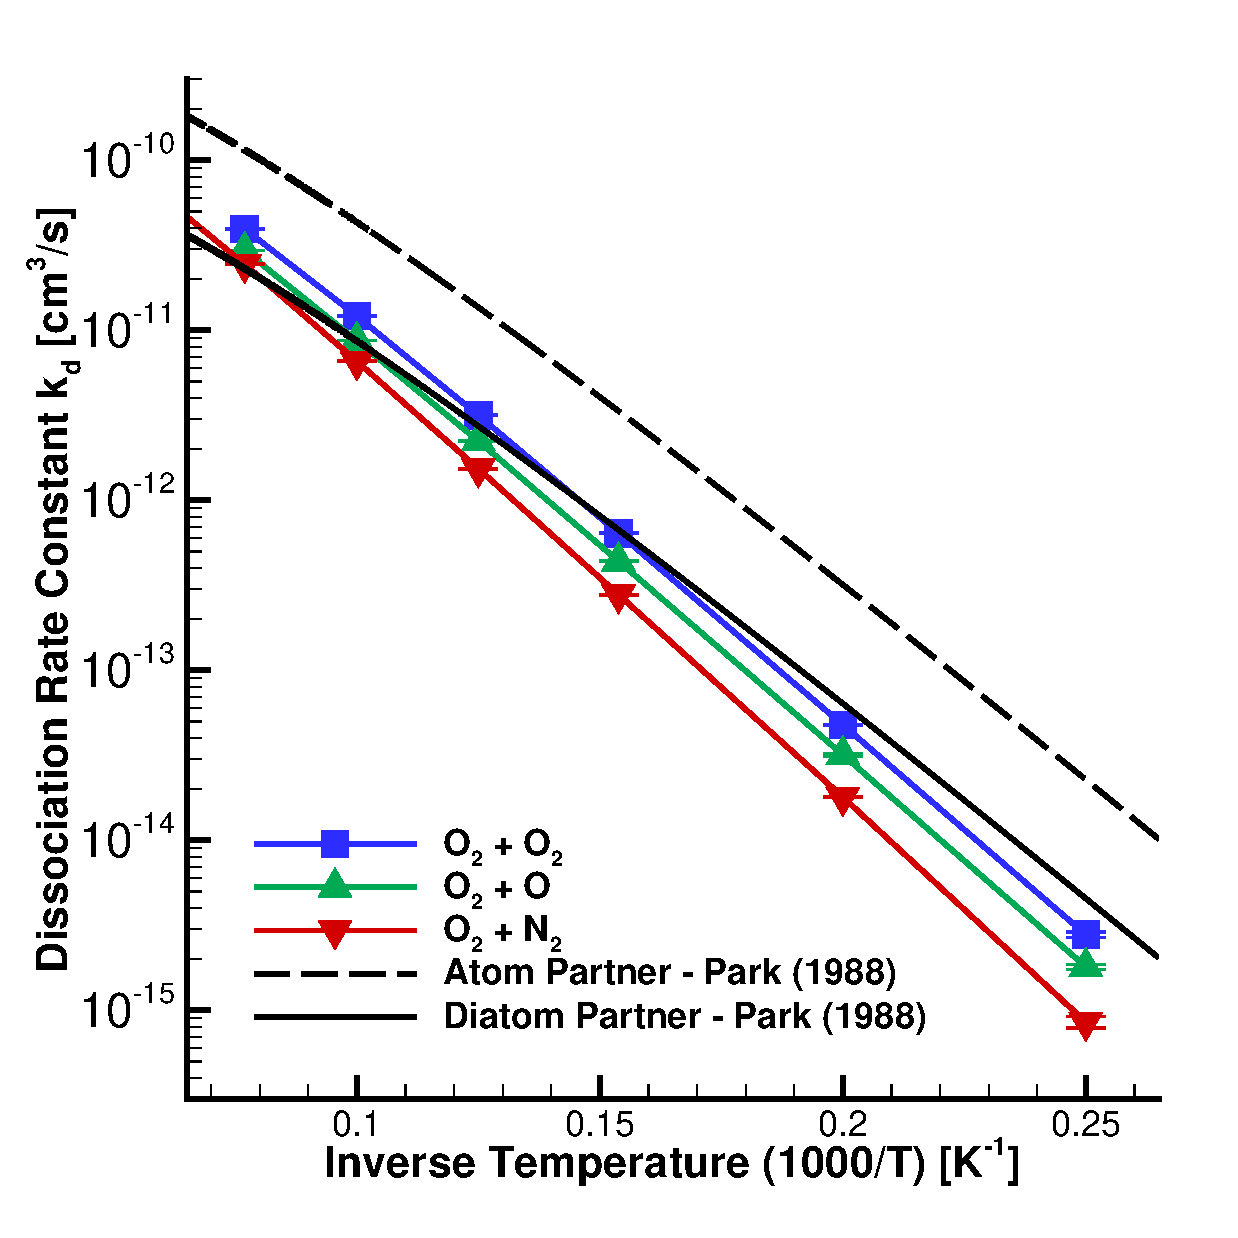
\includegraphics[width=\textwidth]{./figures/O2-Dissoc_AllPartners_Equil.eps}
      \caption{$\Ttr=\Tv$}
   \end{subfigure}
%
   \begin{subfigure}[t]{\twofigwidth\textwidth}
      \centering
      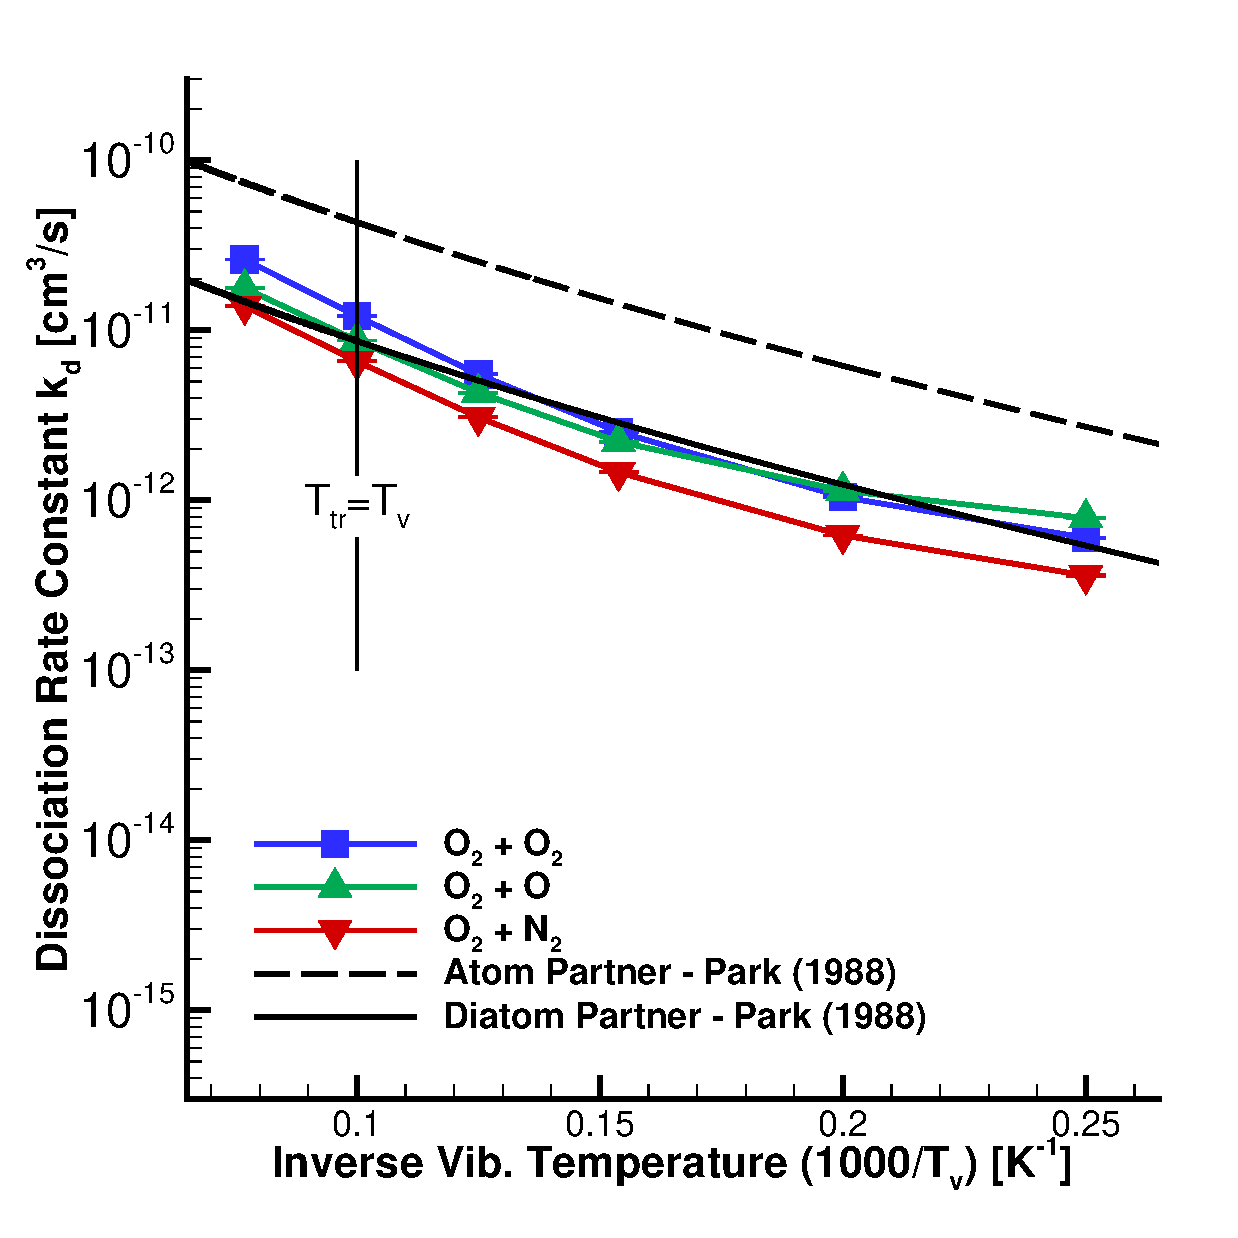
\includegraphics[width=\textwidth]{./figures/O2-Dissoc_AllPartners_Nonequil.eps}
      \caption{$\Ttr=\SI{10000}{\kelvin}$}
   \end{subfigure}
   \caption[Oxygen dissociation with various parameters]
      {Oxygen dissociation rate with collision partners \ce{O2}, \ce{O}, and \ce{N2}
         for the equilibrium and nonequilibrium test set.}
   \label{fig:O2-Dissoc_Rates}
\end{figure}

\begin{figure}[p]
   \centering
   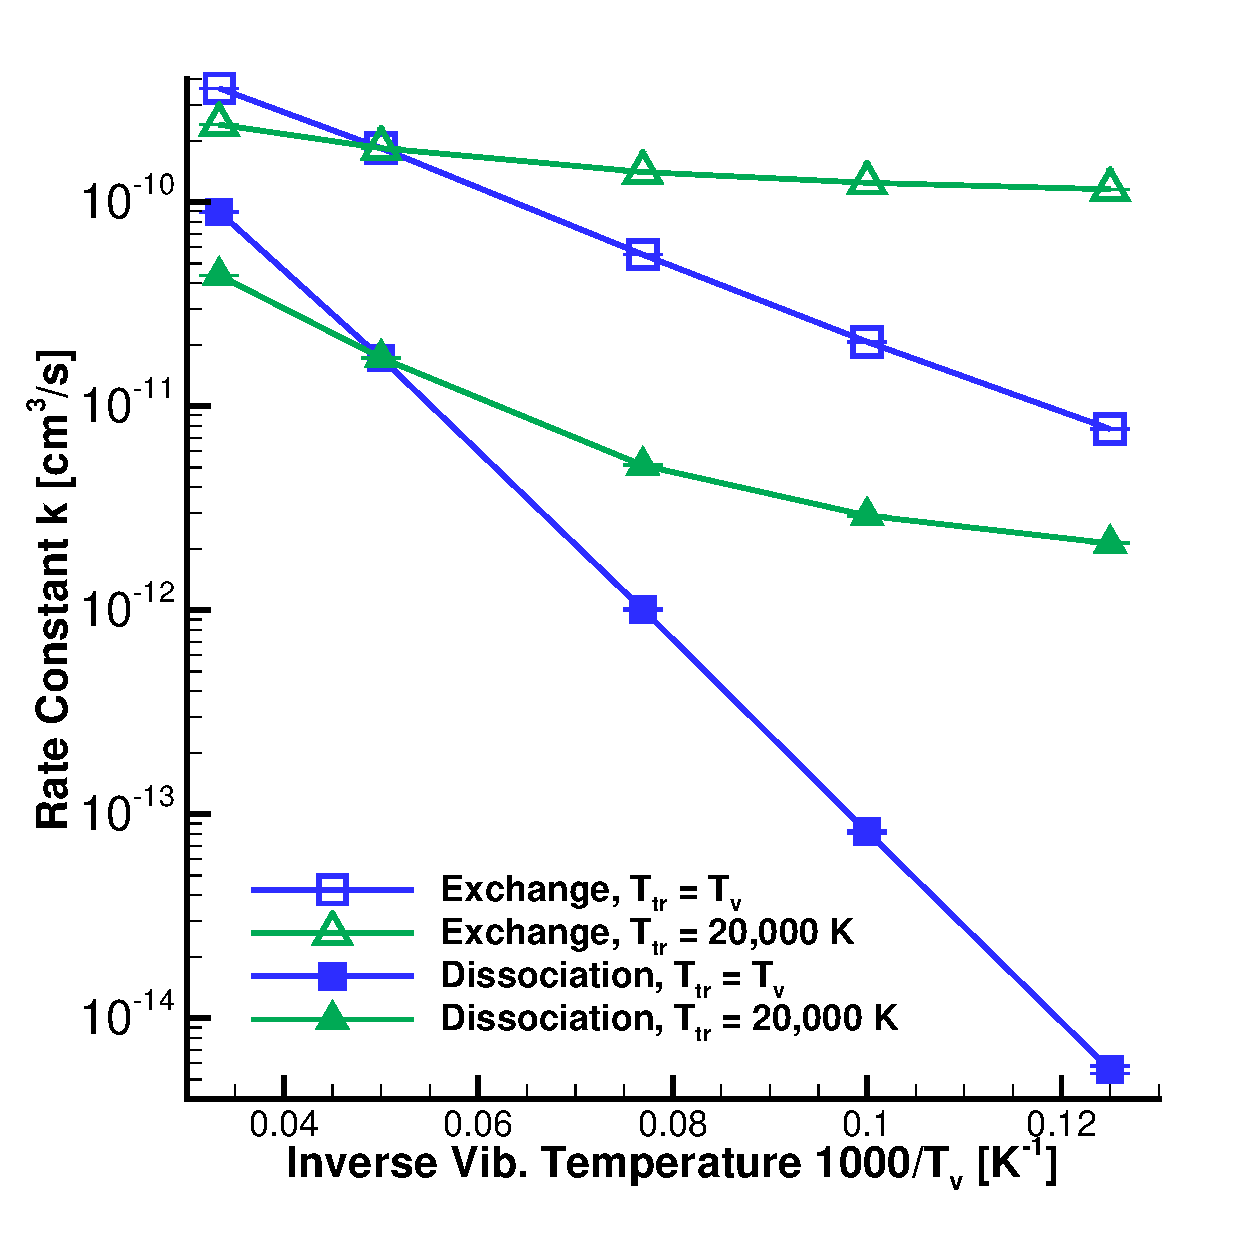
\includegraphics[width=0.48\textwidth]{./figures/N3_Dissoc_vs_Exchange.eps}
   \caption[Exchange and dissociation rates in \ce{N2 + N}]
      {Reaction rate constants for exchange and dissociation in \ce{N2 + N},
      for the equilibrium and nonequilibrium test set.}
   \label{fig:N3_Exchange_Rate}
\end{figure}

For testing, here is a handful of pages filled with junk.
How does the header look, on a page like this?

\lipsum[1-10]

% ===== CONCLUSIONS
% -- Do not bother to make figures relative. Why do you have figures in the conclusions?

\chapter{Conclusions}
\label{sec:Conclusions}

You should definitely have some of these.
Don't write them at the last minute.


% -- Bibliography should be single spaced, so group it from here: https://tex.stackexchange.com/questions/408757/change-linespacing-in-bibliography
% -- Choose new-aiaa for style, could pick others
% -- Formatting here is adapted https://tug.org/pracjourn/2008-1/mori/mori.pdf page 13
\cleardoublepage
\begingroup
\singlespacing
\bibliographystyle{new-aiaa}
\phantomsection
\addcontentsline{toc}{chapter}{\bibname}
\bibliography{Bibliography}
\endgroup

% -- Appendix
\begin{appendices}
\clearpage
\chapter{Nomenclature and Acronyms}
\label{sec:Nomenclature_and_Acronyms}

Several packages could be used for this, including \verb|nomencl|\footnote{https://ctan.org/pkg/nomencl?lang=en}
   and \verb|glossaries|\footnote{https://ctan.org/pkg/glossaries?lang=en}.
However, I prefer to sort in my own order and include sub-headings,
   which I found cumbersome with those tools.
Therefore, this nomenclature section just uses longtable.
Feel free to customize as desired!


% -- Nomenclature
\section{Nomenclature}
\label{sec:Nomenclature}

\begin{longtable*}[l]{l @{\qquad} l}

% -- Latin alphabet (no space here because it's first)
                    \bfseries{Latin}            \\
$b$         &  Impact parameter, \si{\angstrom}                            \\
$T$         &  Temperature, \si{\kelvin}                                   \\
$k$         &  Rate constant, \si{\cm\cubed\per\sec}, OR                   \\
            &  Some other constant, not confusing at all                   \\
$Z$         &  Some duplicate entries to wrap                              \\
$Z$         &  Some duplicate entries to wrap                              \\
$Z$         &  Some duplicate entries to wrap                              \\
$Z$         &  Some duplicate entries to wrap                              \\
$Z$         &  Some duplicate entries to wrap                              \\

% -- Greek alphabet
\addlinespace[5 mm] \bfseries{Greek}            \\
$\ev$       &  Vibrational energy, \si{\eV}, \cref{eqn:ev}                 \\

% -- Subscripts
\addlinespace[5 mm] \bfseries{Subscripts}       \\
d           &  Dissociation                                                \\
e           &  Exchange                                                    \\
t           &  Translational                                               \\
r           &  Rotational                                                  \\
v           &  Vibrational
\end{longtable*}

\section{Acronyms}
\label{sec:Acronyms}

\begin{longtable*}[l]{l @{\qquad} l}
NASA        &  National Aeronautics and Space Administration               \\
PES         &  Potential Energy Surface
\end{longtable*}

\chapter{Tables}
\label{sec:Appendix_Tables}
This is some filler text. Here, there is no section title, so we set the section mark
(for headers) using the command \verb|\sectionmark{Tables for Nitrogen Dissociation}|.
The section number is 0, though, which is a bit unfortunate
   but not a huge problem.

% -- From https://texfaq.org/FAQ-runheadtoobig
\sectionmark{Tables for Nitrogen Dissociation}

\begin{landscape}
% ===== N3 TABLES

% -- Remove one temperature (for equil rename to T) and N4_DUMMY, add rules

% Collected_N3_TX_TvX_table_line_main.dat
\begin{table}[p]
   \caption[\ce{N2 + N}, $\Ttr=\Tv$]
      {Summary statistics for \ce{N2 + N}, equilibrium test set ($\Ttr=\Tv$).}
   \label{tbl:App_N3_EQ}
   \footnotesize
   \begin{tabular}{  S[table-format=5]    S[table-format=3]                   S[table-format=1.3(2)e-2]                                                     S[table-format=-1.3(2)]                                                       S[table-format=-1.3(2)]                                                       S[table-format=1.4(2)e-2]                                                     S[table-format=-1.1(2)e-1]                                                    S[table-format=1.1(2)e-1]                                                  }
      \toprule
      {$T$ $\qty[\si{\kelvin}]$}       &  {$\mathcal{N}$ $\qty[\num{e6}]$} &  {$k_\mathrm{d}$ $\qty[\si{\cm\cubed\per\sec}]$}                            &  {$\left<\Delta\ev\right>_\mathrm{d}$ $\qty[\si{\eV}]$}                     &  {$\left<\Delta\er\right>_\mathrm{d}$ $\qty[\si{\eV}]$}                     &  {$k_\mathrm{e}$ $\qty[\si{\cm\cubed\per\sec}]$}                            &  {$\left<\Delta\ev\right>_\mathrm{e}$ $\qty[\si{\eV}]$}                     &  {$\left<\Delta\er\right>_\mathrm{e}$ $\qty[\si{\eV}]$}                     \\
      \midrule
      8000                             &  240                              &  5.6 \pm 0.2 e-15                                                           &  -7.9 \pm 0.4                                                               &  -1.60 \pm 0.09                                                             &  7.718 \pm 0.005 e-12                                                       &  -3.0 \pm 0.7 e-3                                                           &  2.1 \pm 0.8 e-3                                                            \\
      10000                            &  150                              &  8.20 \pm 0.12 e-14                                                         &  -7.63 \pm 0.13                                                             &  -1.82 \pm 0.04                                                             &  2.0638 \pm 0.0011 e-11                                                     &  -4.6 \pm 0.7 e-3                                                           &  8.8 \pm 0.9 e-3                                                            \\
      13000                            &  60                               &  1.006 \pm 0.007 e-12                                                       &  -7.20 \pm 0.06                                                             &  -2.20 \pm 0.02                                                             &  5.528 \pm 0.003 e-11                                                       &  -5.2 \pm 1.0 e-3                                                           &  0.0104 \pm 0.0013                                                          \\
      20000                            &  18                               &  1.722 \pm 0.006 e-11                                                       &  -6.52 \pm 0.03                                                             &  -2.896 \pm 0.013                                                           &  1.8377 \pm 0.0012 e-10                                                     &  -4.9 \pm 1.6 e-3                                                           &  0.014 \pm 0.002                                                            \\
      30000                            &  18                               &  8.939 \pm 0.014 e-11                                                       &  -5.930 \pm 0.011                                                           &  -3.490 \pm 0.007                                                           &  3.6133 \pm 0.0019 e-10                                                     &  -4.9 \pm 1.5 e-3                                                           &  0.018 \pm 0.002                                                            \\
      \bottomrule
   \end{tabular}
\end{table}

% Collected_N3_T20_TvX_table_line_main.dat
% -- Manually modify equil devib for T20,Tv20
\begin{table}[p]
   \caption[\ce{N2 + N}, $\Ttr=\SI{20000}{\kelvin}$]
      {Summary statistics for \ce{N2 + N}, nonequilibrium test set ($\Ttr=\SI{20000}{\kelvin}$).}
   \label{tbl:App_N3_NEQ}
   \footnotesize
   \begin{tabular}{  S[table-format=5]    S[table-format=2]                   S[table-format=1.3(2)e-2]                                                     S[table-format=-1.3(2)]                                                       S[table-format=-1.3(2)]                                                       S[table-format=1.4(2)e-2]                                                     S[table-format=-1.4(2)]                                                       S[table-format=-1.4(2)]                                                    }
      \toprule
      {$\Tv$ $\qty[\si{\kelvin}]$}     &  {$\mathcal{N}$ $\qty[\num{e6}]$} &  {$k_\mathrm{d}$ $\qty[\si{\cm\cubed\per\sec}]$}                            &  {$\left<\Delta\ev\right>_\mathrm{d}$ $\qty[\si{\eV}]$}                     &  {$\left<\Delta\er\right>_\mathrm{d}$ $\qty[\si{\eV}]$}                     &  {$k_\mathrm{e}$ $\qty[\si{\cm\cubed\per\sec}]$}                            &  {$\left<\Delta\ev\right>_\mathrm{e}$ $\qty[\si{\eV}]$}                     &  {$\left<\Delta\er\right>_\mathrm{e}$ $\qty[\si{\eV}]$}                     \\
      \midrule
      8000                             &  90                               &  2.122 \pm 0.007 e-12                                                       &  -1.333 \pm 0.008                                                           &  -6.71 \pm 0.03                                                             &  1.1541 \pm 0.0004 e-10                                                     &  0.9139 \pm 0.0007                                                          &  -0.5638 \pm 0.0011                                                         \\
      10000                            &  60                               &  2.903 \pm 0.011 e-12                                                       &  -2.292 \pm 0.014                                                           &  -6.11 \pm 0.03                                                             &  1.2434 \pm 0.0005 e-10                                                     &  0.7583 \pm 0.0009                                                          &  -0.4785 \pm 0.0013                                                         \\
      13000                            &  60                               &  5.118 \pm 0.015 e-12                                                       &  -4.011 \pm 0.017                                                           &  -4.878 \pm 0.019                                                           &  1.4031 \pm 0.0006 e-10                                                     &  0.5136 \pm 0.0009                                                          &  -0.3338 \pm 0.0013                                                         \\
      20000                            &  18                               &  1.722 \pm 0.006 e-11                                                       &  -6.52 \pm 0.03                                                             &  -2.896 \pm 0.013                                                           &  1.8377 \pm 0.0012 e-10                                                     &  -0.0049 \pm 0.0016                                                         &  0.014 \pm 0.002                                                            \\
      30000                            &  60                               &  4.371 \pm 0.005 e-11                                                       &  -7.565 \pm 0.010                                                           &  -2.017 \pm 0.003                                                           &  2.3971 \pm 0.0008 e-10                                                     &  -0.4721 \pm 0.0009                                                         &  0.3574 \pm 0.0011                                                          \\
      \bottomrule
   \end{tabular}
\end{table}
\end{landscape}

\end{appendices}


\end{document}

